\documentclass{standalone}
    %
    \usepackage{tikz,xcolor}
    \usetikzlibrary{shapes.geometric,arrows,positioning,fit}
    
\begin{document}
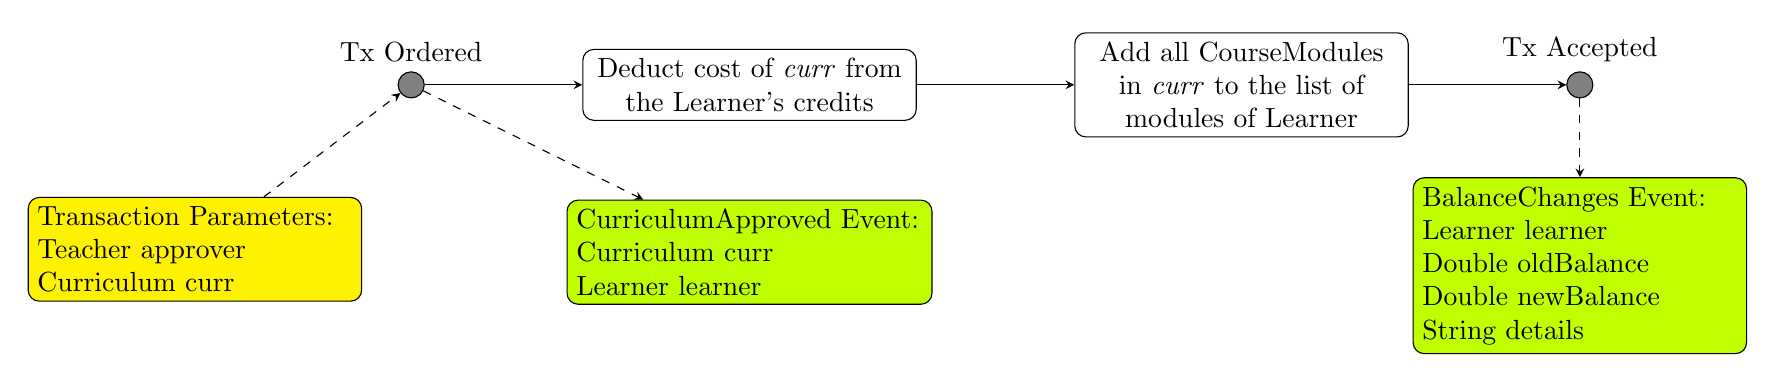
\begin{tikzpicture}[>=stealth,every node/.style={shape=rectangle,draw,rounded corners},]
	% create the nodes
    \node (param)[text width=4cm, fill=yellow]{Transaction Parameters:\\Teacher approver\\ Curriculum curr};
	\node (start)[above right = 1.3cm and 0.5cm of param, shape=circle, fill=gray, label=above:Tx Ordered] {};    
    \node (c1) [right = 2cm of start, text width=4cm, align=center]{Deduct cost of \textit{curr} from the Learner's credits};
	\node (c2) [right = 2cm of c1, text width=4cm, align=center]{Add all CourseModules in \textit{curr} to the list of modules of Learner};
	\node (stop1)[right = 2cm of c2, shape=circle, fill=gray, label=above:Tx Accepted] {};
    \node (event1)[below =of c1, text width=4.4cm, fill=lime]{CurriculumApproved Event:\\ Curriculum curr \\ Learner learner };        
    \node (event2)[below =of stop1, text width=4cm, fill=lime]{BalanceChanges Event:\\ Learner learner \\ Double oldBalance \\ Double newBalance \\ String details};    

	% connect the nodes
	\draw[->, dashed] (param) to (start);
	\draw[->] (start) to (c1);
    \draw[->] (c1) to (c2);        
    \draw[->] (c2) to (stop1);        
	\draw[->, dashed] (start) to (event1);    
	\draw[->, dashed] (stop1) to (event2);
    
\end{tikzpicture}
\end{document}
